\documentclass{article}

\usepackage{a4wide}
\usepackage[utf8]{inputenc}
\usepackage[T1]{fontenc}
\usepackage{natbib}
\usepackage[french]{babel}
\usepackage[babel=true]{csquotes} % guillemets français
\usepackage{graphicx}
\graphicspath{{Images/}}
\usepackage{color}
\usepackage{hyperref}
\hypersetup{colorlinks,linkcolor=,urlcolor=blue}

\usepackage{amsmath}
\usepackage{amssymb}


\title{Rapport de projet iOS et Android : Survivor}
\author{\'Nativel Emmanuel et Hoarau Raphael,  L3 informatique}
\date{\today}

\begin{document}

\maketitle % pour écrire le titre


%% Le résumé:
\begin{abstract}
  Présentation de notre application nommée Survivor,  un jeu de défense en 2D pour mobile développé sous android et iOS dans le cadre de l'UE programmation mobile en L3 informatique.
\end{abstract}

\section{Introduction}
\label{section:introduction}

Dans le cadre de l'UE programmation mobile en L3 informatique, nous devons développer une application sous Android et iOS en respectant plusieurs contraintes. Celle-ci doit proposer plusieurs écrans affichés correctement en mode portrait et paysage et quelle que soit la taille de l'appareil sur lequel l'application est lancée. L'un de ces écrans doit proposer un menu permettant de lancer une partie ou de consulter l'historique des scores des parties précédentes classés du score le plus élevé au plus faible. Le joueur doit également pouvoir supprimer un score de la liste. De plus ces données doivent être enregistrées de manière persistante sur l'une des deux plateformes. Nous avons choisi de le faire sous Android. Enfin, à la fin d'une partie, un écran doit apparaître afin d'afficher le score du joueur et de lui demander de saisir un nom à associer à ce score.
Afin de répondre à ces différentes contraintes, nous avons décidé de développer un jeu de défense en 2D que nous avons appelé Survivor.

Dans un premier temps, nous allons vous présenter le fonctionnement du jeu ainsi que son architecture. Puis, nous vous exposerons quelques points essentiels du développement de ce jeu, de l'animation des Sprites à la génération des monstres, en passant par la détection des collisions. Enfin, nous verrons que même si le jeu doit être identique sur les deux plateformes, il reste tout de même quelques différences notables. Et pour terminer, nous vous expliquerons les principales difficultés que nous avons rencontrées au long de ce projet.

\section{Description de l'application}

Survivor est un jeu mobile en 2D. L’utilisateur incarne un personnage placé au centre d'un chemin sur lequel des monstres vont apparaître à chaque extrémité pour charger le joueur dans le but de le tuer. L’objectif est de survivre le plus longtemps possible aux vagues de monstres envoyées par la droite et la gauche de la carte. 
Il y a trois types de monstres qui peuvent être générés. Le plus faible, qui peut être tué en un seul coup de projectile, est le gobelin. Il y a aussi le golem, qui nécessite deux coups de projectiles avant de mourir, et enfin il y a le chevalier, le monstre le plus résistant, qui en demande trois.
Cependant, chaque monstre a une probabilité d'être généré qui est différente. Le gobelin a cinq chances sur dix d'être généré, le golem quatre chances sur dix et le chevalier que deux chances sur dix.
Concernant le score, il est incrémenté de la valeur du monstre tué à chaque fois qu'un monstre meurt, sachant qu'un gobelin a une valeur de un, un golem une valeur de deux et un chevalier une valeur de trois.

\section{Architecture générale de l'application}
\label{section:architecture}

Notre application contient quatre écrans : le menu, la scène de jeu, l'écran de GameOver et l'historique des scores.
Pour modéliser les différents objets de notre jeu, nous avons décidé de créer les classes suivantes :
\begin{itemize}
\item La classe \textbf{GameScene} : Représente notre scène de jeu, l'environnement dans lequel se trouvent nos différents objets.
\item La classe \textbf{Player} : Représente le joueur.
\item La classe \textbf{Monster} : Représente un monstre. Le type du monstre est donné en argument.
\item La classe \textbf{Projectile} : Représente un projectile tiré par le joueur.
\item La classe \textbf{MonsterGenerator} : S'occupe de générer des monstres dans une direction donnée.
\end{itemize}

\section{Fonctionnement d'une partie}
Pour une partie, nous avons donc besoin d'une instance de GameScene qui contiendra deux instances de MonsterGenerator, une à droite et une à gauche qui eux-mêmes génèrent des instances de différents types de Monster.
Notre GameScene a également une instance de Player qui tire des instances de projectiles dans la direction où l'utilisateur appuie.

\section{Captures d'écran}
\label{section:capture}

Toutes les images que nous avons utilisées pour notre jeu sont libres de droit et ont été prises sur craftPix\cite{craftPix}. 
\bigskip

Ecran du menu : 
\begin{center}
  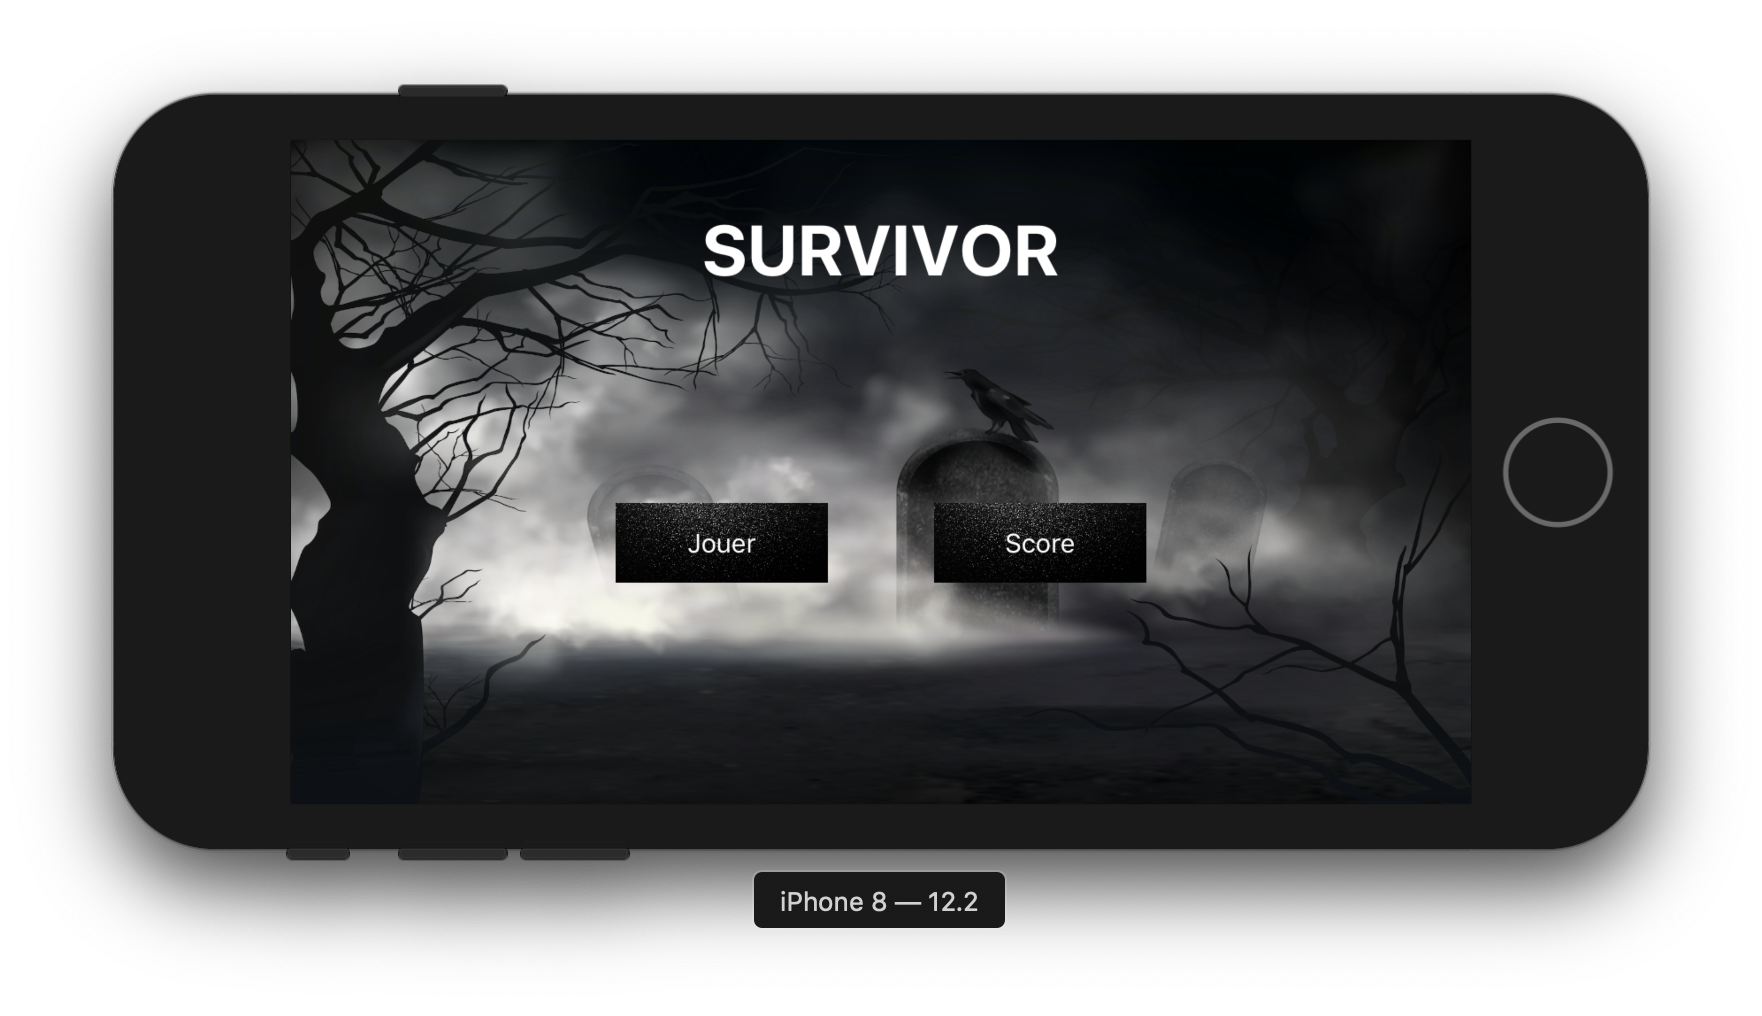
\includegraphics[scale=0.4]{menu.png}
\end{center}

\cleardoublepage

Ecran de jeu : 
\begin{center}
  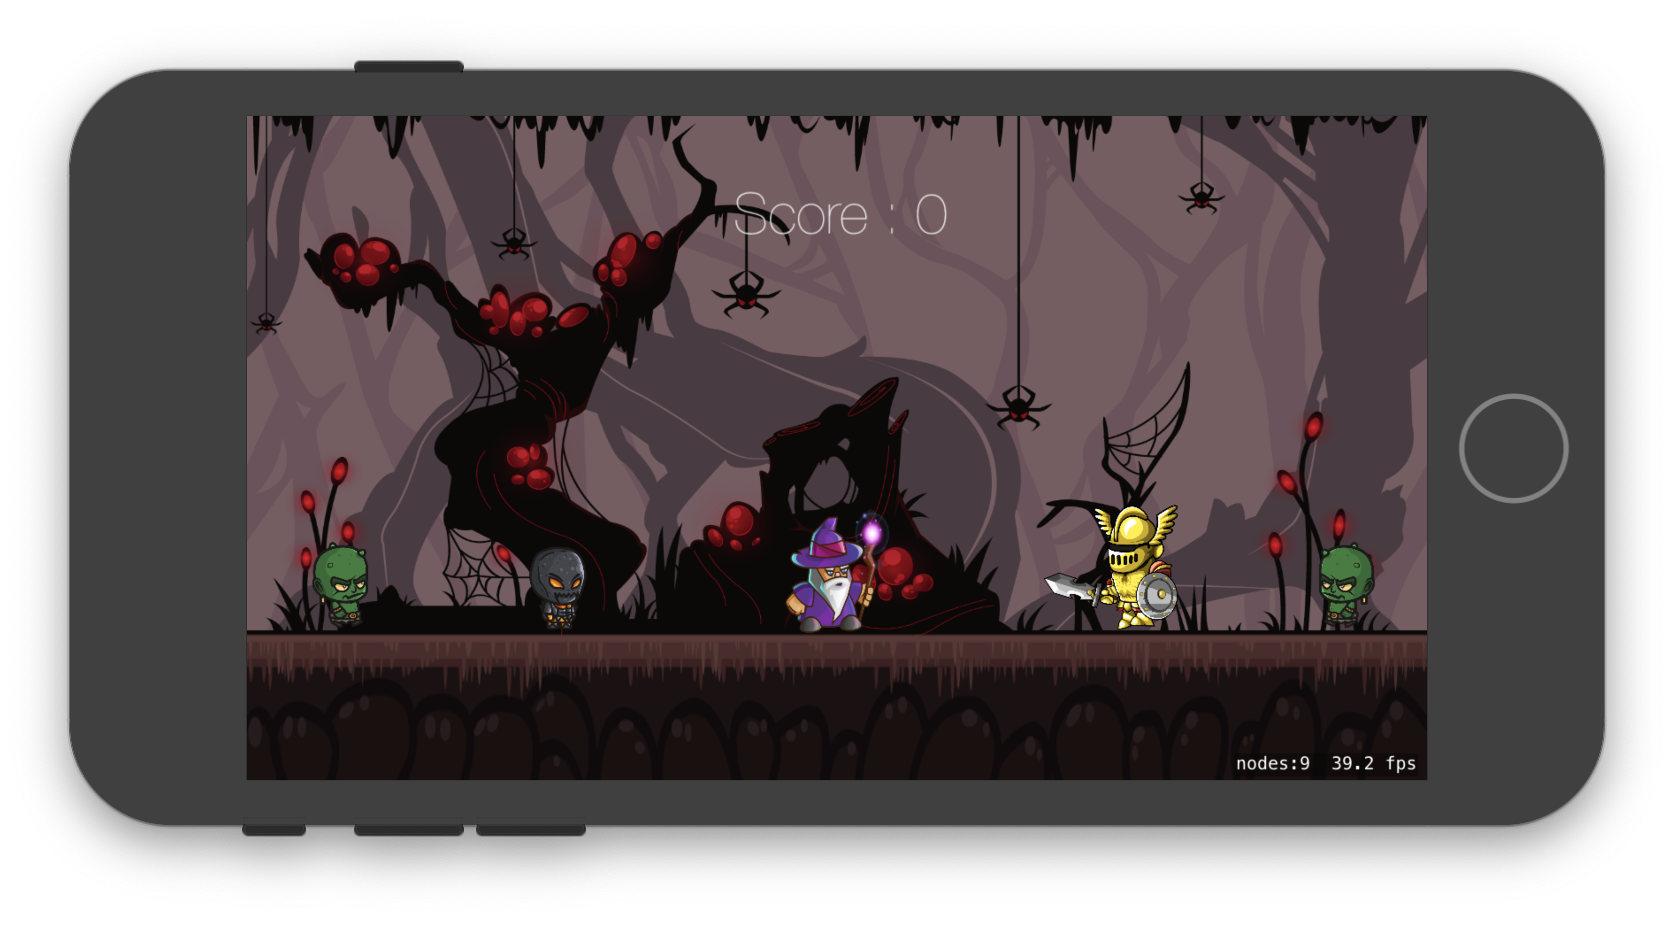
\includegraphics[scale=0.4]{jeu.png}
\end{center}

Ecran Game Over : 
\begin{center}
  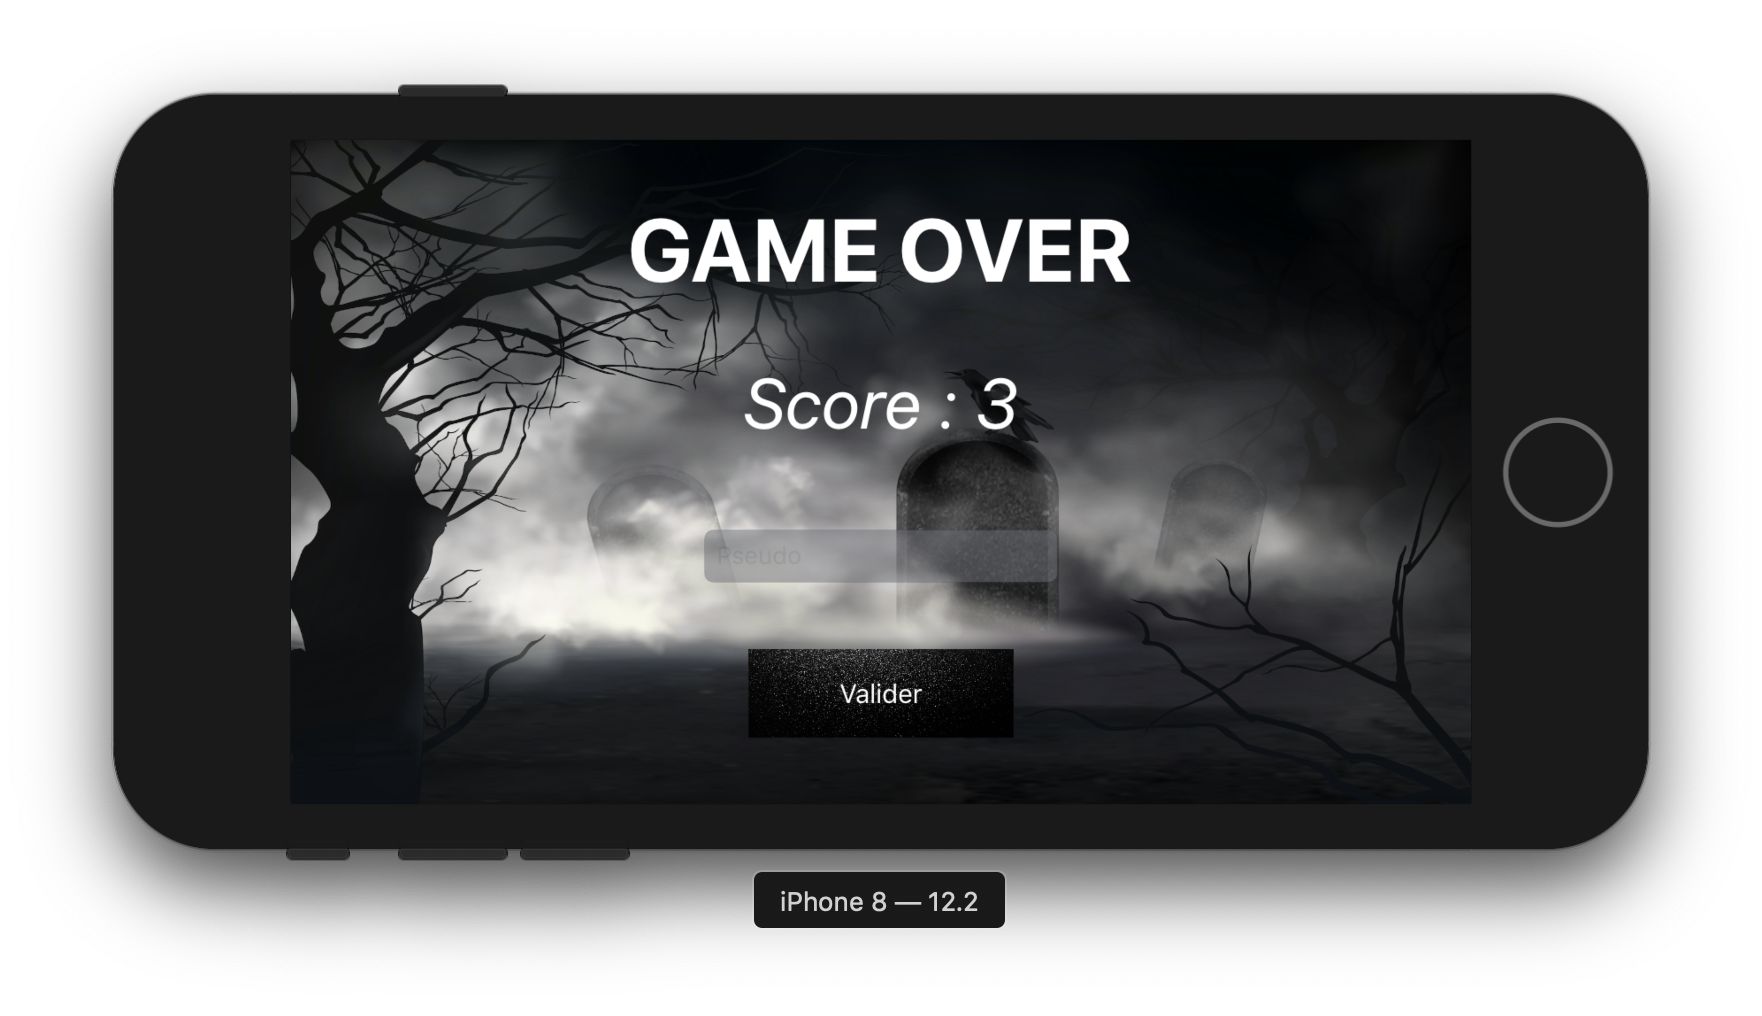
\includegraphics[scale=0.4]{gameover.png}
\end{center}

Ecran des scores  sous iOS: 
\begin{center}
  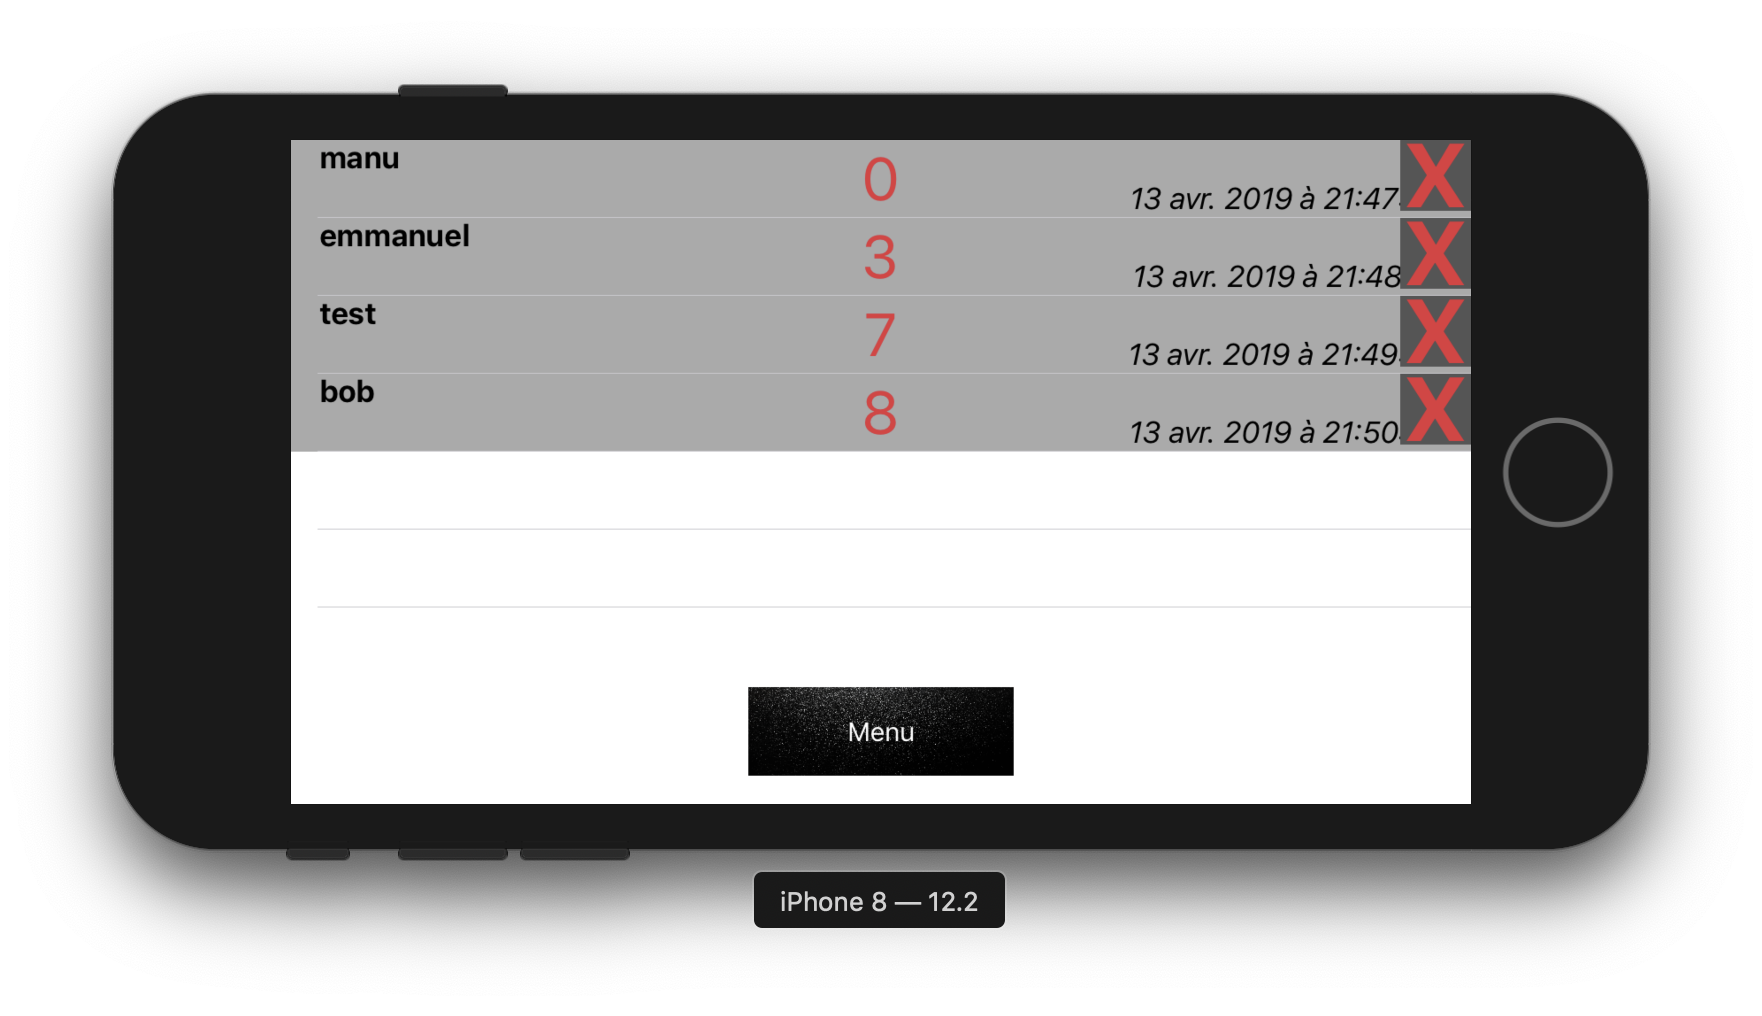
\includegraphics[scale=0.3]{score.png}
\end{center}

\cleardoublepage

\section{Animations}

\subsection{Sous iOS : SKAction}

	Sous iOS, l'animation des sprites était très intuitive grâce à la librairie Sprite Kit.
Nous avons commencé par créer nos animations dans le fichier Action.sks. Pour chaque animation il faut d'abord créer un objet AnimateWithTextures, puis faire glisser les images qui constituent l'animation à l'intérieur et enfin ajouter une durée à l'animation ainsi qu'un nombre de répétitions (qui peut être infini).
    
    Ensuite grâce à la classe SKAction, nous pouvons lancer ces animations et même effectuer des actions supplémentaires en parallèle de l'animation grâce à SKAction.group() ou alors sous forme de suite d'actions avec SKAction.sequence().
    \bigskip
    
    Comme exemple, voici un extrait du code de la fonction die() du joueur :
    
    \begin{verbatim}
        let die:SKAction = SKAction(named: self.direction+"_DiePlayer")!
        let finish:SKAction = SKAction.run {
            self.removeFromParent()
            self.gameOver = true
        }
        let seq:SKAction = SKAction.sequence([die, finish])
        self.run(seq)
    \end{verbatim}
    
    Dans notre exemple, nous définissons trois SKAction. Le premier, nommé "die" contient l'animation que nous avons placée dans le fichier Action.sks. La seconde, "finish" est un groupe de code à exécuter. Enfin, la dernière SKAction "seq" est notre séquence, elle permet de faire en sorte que l'action "die" soit exécutée en premier, puis vient l'exécution de "finish". Pour terminer, nous lançons l'exécution de "seq" avec la méthode run().
    \bigskip
    
    Nous avons également utilisé l'action SKAction.group() pour gérer nos animations. A titre d'exemple, voici la fonction move() de la classe Projectile : 
    
    \begin{verbatim}
    func move(sens:CGFloat, animation:String){
        let moveAnimation:SKAction = SKAction(named: animation)!
        let moveAction:SKAction = SKAction.moveTo(x: sens * (self.scene?.size.width)!, duration: 0.8)
        let group:SKAction = SKAction.group([moveAnimation, moveAction])
        self.run(group)
    }
    \end{verbatim}
    
    Ici, l'action "moveAnimation" récupère notre animation du projectile et nous avons aussi "moveAction" qui est l'action qui permet de déplacer le projectile. 
    Dans ce cas, nous voulons que le déplacement et l'animation se produisent en même temps. Pour cela, nous avons donc utilisé l'action "group".
        
        \subsection{Sous Android : Animations et AnimationManager}
Sous android, les animations sont gérées par la classe Animation qui prend en paramètre un tableau d'images, la durée de l'animation et un booléen qui détermine si l'animation doit se répéter indéfiniment ou pas. Les animations sont ensuite gérées par un AnimationManager qui contient un tableau d'animations. 

\cleardoublepage
       
 \section{Détection des collisions}

\subsection{Sous iOS : categoryBitMask, contactTest et collisionBitMask}
Sous iOS, chaque sprite a un categoryBitMask qui l'identifie. C'est un mot sur 32 bit. Dans notre cas, le sol, le joueur, les monstres et les projectiles ont des categoryBitMask différents car on veut qu'ils puissent entrer en contact.
\begin{verbatim}
        let playerCategory:UInt32 = 1 << 0      	// ...0000001
        let monsterCategory:UInt32 = 1 << 1     	// ...0000010
        let projectileCategory:UInt32 = 1 << 2  	// ...0000100
        let groundCategory:UInt32 = 1 << 3       // ...0001000
\end{verbatim}

Chaque sprite a également un contactTestBitMask qui fait référence aux objets avec lesquels le sprite peut avoir un contact. A ne pas confondre avec les collisions, car on peut détecter un contact sans qu'il y ait collision entre les deux objets.
En revanche, le collisionBitMask fait référence à un contact physique entre deux objets.
Prenons l'exemple de la classe Monster dans notre jeu. 
Nous voulons détecter lorsqu'un monstre entre en contact avec le joueur ou avec un projectile et lorsqu'il entre en collision avec le sol pour pas qu'il passe à travers. Nous avons donc : 
\begin{verbatim}
        self.physicsBody?.categoryBitMask = monsterCategory
        self.physicsBody?.collisionBitMask = groundCategory
        self.physicsBody?.contactTestBitMask = projectileCategory | playerCategory
\end{verbatim}

Enfin, une fois tous les sprites paramétrés correctement, c'est la fonction didBegin(contact) qui s'occupe de détecter les contacts. Le paramètre "contact" de la fonction est doté des attributs contact.bodyA et contact.bodyB qui permettent d'identifier les deux objets qui sont entrés en contact. Il suffit donc de récupérer le categoryBotMask de bodyA et bodyB pour savoir de quel objet il s'agit. 

Par exemple, pour tester les contacts entre le joueur et un monstre, nous avons : 

\begin{verbatim}
 func didBegin(_ contact: SKPhysicsContact) {
 		if(contact.bodyA.categoryBitMask == playerCategory && contact.bodyB.categoryBitMask == monsterCategory){
            
            let monster:Monster = contact.bodyB.node as! Monster

            monster.attack()
            player.die()
        }
 }
\end{verbatim}

\subsection{Sous Android : comparaison des coordonnées}
Sous Android, chaque sprite est assimilé à un rectangle. De ce fait, pour savoir si deux objets entrent en collision, il suffit de déterminer si leurs rectangles respectifs se touchent. Cela est fait par la méthode Rect.intersects(rectA, rectB) qui retourne true si rectA et rectB se touchent.

Par exemple, dans la classe Monster, pour tester si  il y a collision avec le joueur :
\begin{verbatim}
        public boolean playerCollide(Player player){
            return Rect.intersects(rectangle, player.getRectangle());
        }
\end{verbatim}

\cleardoublepage

\section{Génération des monstres}
La génération des monstres est effectuée par la classe MonsterGenerator. Cette classe contient une liste de monstres et un nombre maximum de monstres présents sur la map et qui ont été générés par ce générateur de monstres. Elle contient aussi une variable qui correspond à une distance limite que doit avoir passé le dernier monstre généré pour que la génération d'un nouveau monstre soit autorisée.

L'algorithme de génération est donc le suivant : 
Si la liste de monstre est vide alors on génère un monstre. 
Sinon, si la taille de la liste est inférieure au nombre maximum de monstre et que le dernier monstre généré a dépassé la limite, alors on génère un monstre.

\begin{center}
  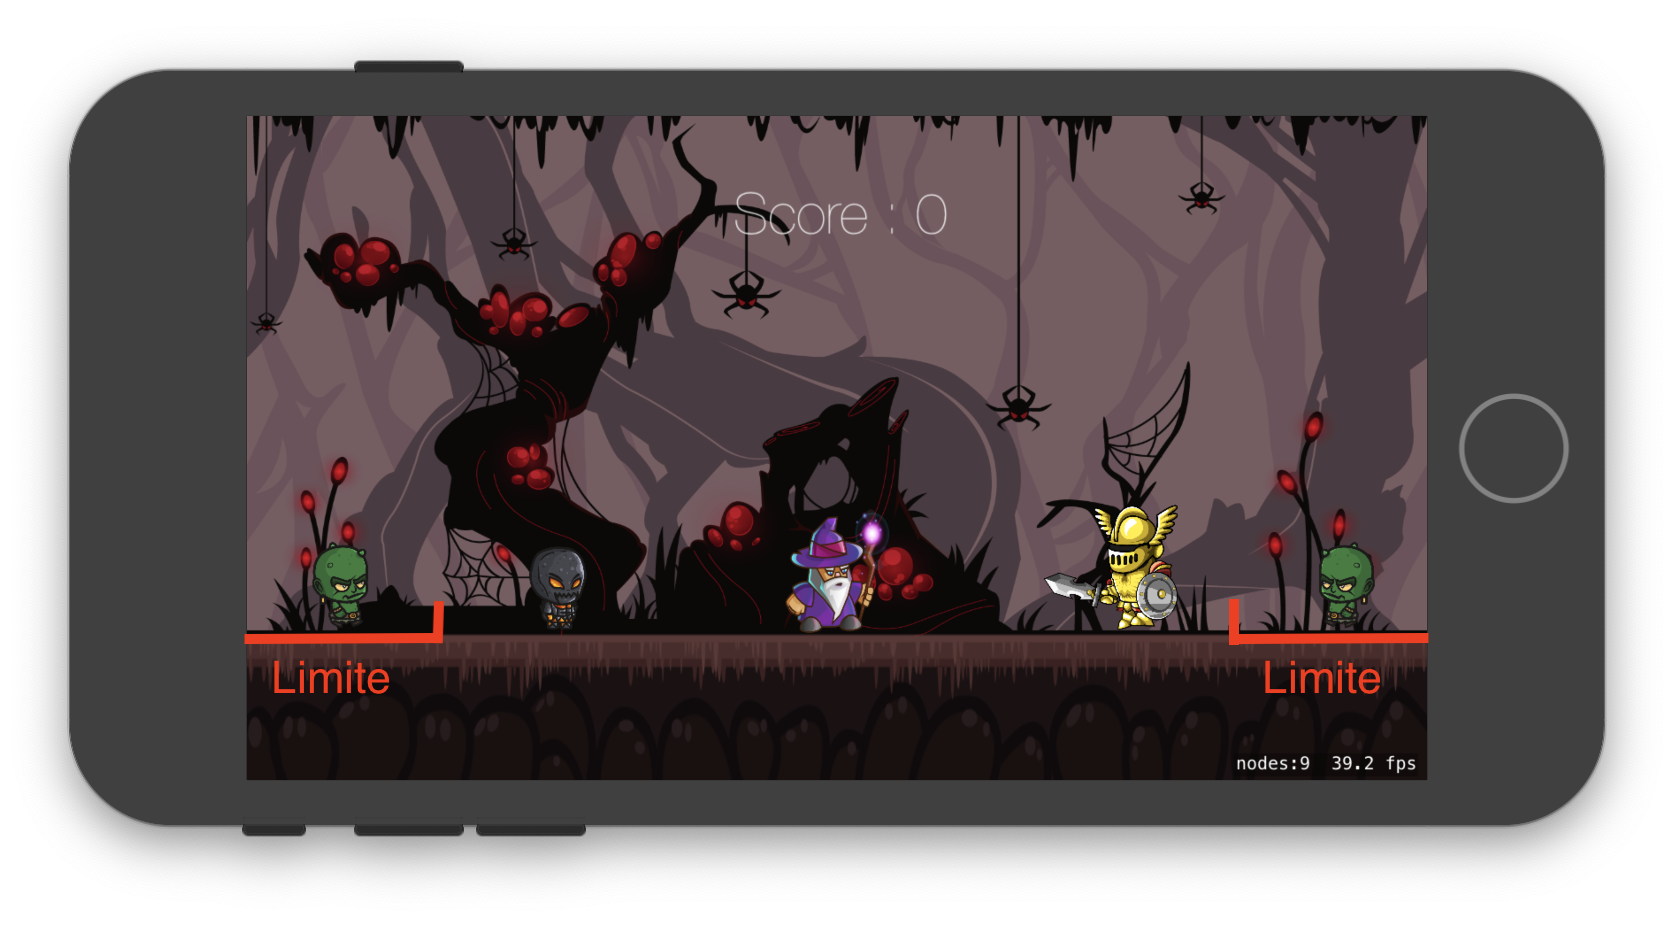
\includegraphics[scale=0.4]{limite.png}
\end{center}

\section{Les différences entre Android et iOS}
Même si le jeu est le même sur Android et sur iOS, sur certains points nous n'avons pas réussi à reproduire la même chose à l'identique sur les deux plateformes. 
Notamment au niveau des paramètres du gameplay : la vitesse des monstres, la vitesse de tir du joueur, ou encore la limite permettant de générer des monstres. Nous ne pouvons pas certifier que ces paramètres soient complètement identiques sur les deux plateformes.
D'autres différences sont aussi relevables. Comme la méthode de détection des collisions, qui est faite en utilisant la physique sur iOS et en comparant simplement les coordonnées des sprites sur android. Il y a aussi le fait que les données soient persistantes uniquement sur android.
Enfin, au niveau visuel, il y a aussi quelques différences. Premièrement au niveau des animations. Les animations des monstres ont été supprimées sur android à cause d'un problème de mémoire décrit plus bas. Puis, le design de l'écran de score est différent sur iOS et sur Android à cause d'un soucis de temps.

\section{Difficultés rencontrées}
\label{section:difficultées}
Nous avons rencontré plusieurs difficultés au cours du développement. Premièrement au niveau de la mise en place de la game loop et des animations des sprites sous Android. En effet, nous avons dû mettre en place un thread qui joue le rôle de game loop, grâce à un tutoriel\cite{tutoGameLoop}. En ce qui concerne les animations, android impose une limitation de mémoire à notre application. Par conséquent nous avons dû supprimer les animations des monstres pour cette plateforme.
En revanche, l'utilisation de la librairie SpriteKit sur iOS rend l'animation des sprites très intuitive grâce aux SKActions et au fichier Actions.sks. De plus, la game loop est générée automatiquement à la création du projet par une simple fonction update.
Le problème a été que nous avons commencé par développer le jeu sous iOS et il a été difficile de le reproduire sous android sans librairie équivalente à SpriteKit.

Un autre problème majeur que nous avons rencontré a été le changement d'écran, plus spécialement pour sortir de la scène de jeu (SurfaceView sur Android ou GameScene sur iOS) et aller vers une scène "normale" de type ViewController sur iOS ou Avtivity sur Android.

Enfin, nous avons également un problème que nous n'avons pas réussi à résoudre au niveau de l'animation d'attaque du joueur. Nous n'avons pas réussi à redimensionner les images de cette animation afin que la taille du joueur ne change pas lorsqu'il attaque.

\section{Conclusion}
\label{section:conclusion}

En conclusion, nous avons trouvé que la programmation sous iOS était beaucoup plus intuitive que sous Android, notamment grâce au langage Swift qui est plûtot simple à comprendre, mais aussi grâce à la librairie SpriteKit qui facilite grandement le développement des jeux 2D.
Pour terminer, nous pourrions imaginer différentes améliorations et évolutions à notre jeu. Comme l'ajout de sorts spéciaux pour le joueur, ou des sorts générés par la carte et qui doivent être esquivés par le joueur, ou encore un déplacement vertical du joueur afin de rendre le jeu plus dynamique.

\bibliographystyle{plain}
\bibliography{ma_biblio}

\end{document}
